\documentclass[]{article}
\usepackage[margin=1.5in]{geometry}
\usepackage{lmodern}
\usepackage{amssymb,amsmath}
\usepackage[backend=biber,natbib=true,style=authoryear-comp,citestyle=authoryear]{biblatex}
\usepackage{ifxetex,ifluatex}
\usepackage{fixltx2e} % provides \textsubscript
\ifnum 0\ifxetex 1\fi\ifluatex 1\fi=0 % if pdftex
  \usepackage[T1]{fontenc}
  \usepackage[utf8]{inputenc}
\else % if luatex or xelatex
  \ifxetex
    \usepackage{mathspec}
  \else
    \usepackage{fontspec}
  \fi
  \defaultfontfeatures{Ligatures=TeX,Scale=MatchLowercase}
\fi
% use upquote if available, for straight quotes in verbatim environments
\IfFileExists{upquote.sty}{\usepackage{upquote}}{}
% use microtype if available
\IfFileExists{microtype.sty}{%
\usepackage[]{microtype}
\UseMicrotypeSet[protrusion]{basicmath} % disable protrusion for tt fonts
}{}
\PassOptionsToPackage{hyphens}{url} % url is loaded by hyperref
\usepackage[unicode=true]{hyperref}
\usepackage{xcolor}
\hypersetup{
            colorlinks,
            linkcolor={red!50!black},
		    citecolor={black},
		    urlcolor={blue!50!black},
            pdftitle={Civilizational filters and distribution of values in the multiverse},
            pdfborder={0 0 0},
            breaklinks=true}
\urlstyle{same}  % don't use monospace font for urls
\usepackage{graphicx,grffile}
\makeatletter
\def\maxwidth{\ifdim\Gin@nat@width>\linewidth\linewidth\else\Gin@nat@width\fi}
\def\maxheight{\ifdim\Gin@nat@height>\textheight\textheight\else\Gin@nat@height\fi}
\makeatother

\bibliography{references_filters.bib}  % The name of your .bib file.

% Scale images if necessary, so that they will not overflow the page
% margins by default, and it is still possible to overwrite the defaults
% using explicit options in \includegraphics[width, height, ...]{}
\setkeys{Gin}{width=\maxwidth,height=\maxheight,keepaspectratio}
\IfFileExists{parskip.sty}{%
\usepackage{parskip}
}{% else
\setlength{\parindent}{0pt}
\setlength{\parskip}{6pt plus 2pt minus 1pt}
}
\setlength{\emergencystretch}{3em}  % prevent overfull lines
\providecommand{\tightlist}{%
  \setlength{\itemsep}{0pt}\setlength{\parskip}{0pt}}
\setcounter{secnumdepth}{0}
% Redefines (sub)paragraphs to behave more like sections
\ifx\paragraph\undefined\else
\let\oldparagraph\paragraph
\renewcommand{\paragraph}[1]{\oldparagraph{#1}\mbox{}}
\fi
\ifx\subparagraph\undefined\else
\let\oldsubparagraph\subparagraph
\renewcommand{\subparagraph}[1]{\oldsubparagraph{#1}\mbox{}}
\fi

% set default figure placement to htbp
\makeatletter
\def\fps@figure{htbp}
\makeatother


\title{Civilizational filters and distribution of values in the multiverse\\ \vspace{5mm} \small{Complementary notes on multiverse-wide superrationality}}
\author{Caspar \"Osterheld}
\date{}

\begin{document}
\maketitle

One factor that might affect the distribution of values in the
multiverse is the possibility of civilizational collapse or extinction.

Given the number of stars in our galaxy and the fact that it is common
for stars to have planets, many
\href{https://en.wikipedia.org/wiki/Planetary_habitability}{\emph{habitable}}
planets probably exist in the galaxy, some of which are probably older
than Earth. If evolution had happened on these other planets in a
similar way as it happened on Earth, intelligent life ought to have
developed on at least some of those planets. And at least some of those
lifeforms ought, in turn, to have built technological civilizations
capable of sending detectable signals into space. Given these
assumptions and the immense size and age of our galaxy, not only should
many such civilizations already have arisen in our corner of the
universe; we should be able to detect their signals or even observe them
directly (see the
\href{https://en.wikipedia.org/wiki/Drake_equation}{\emph{Drake
equation}}). And yet, we do not. This is the
\href{https://en.wikipedia.org/wiki/Fermi_paradox}{\emph{Fermi paradox}}
-- the discrepancy
between estimates of the probability that we can somehow observe
intelligent life in our galaxy, and our lack of any such observations.
Various
\href{https://en.wikipedia.org/wiki/Fermi_paradox\#Hypothetical_explanations_for_the_paradox}{\emph{explanations
of the Fermi paradox}}
\href{http://reducing-suffering.org/ranking-explanations-of-the-fermi-paradox/}{\emph{have
been proposed}} \parencite{Webb2015-vi}. It could be that
\href{https://en.wikipedia.org/wiki/Rare_Earth_hypothesis}{\emph{Earth-like
or otherwise habitable planets are actually very rare}}, or that humans
are indeed just the first intelligent civilization to arise in the
galaxy. Perhaps
\href{https://en.wikipedia.org/wiki/Fermi_paradox\#Human_beings_have_not_existed_long_enough}{\emph{we
have not existed long enough}} to detect or be detected by
extraterrestrials. Maybe we are
\href{https://en.wikipedia.org/wiki/Fermi_paradox\#Humans_are_not_listening_properly}{\emph{bad
at detecting alien civilizations}},
p\href{https://en.wikipedia.org/wiki/Fermi_paradox\#Humans_are_not_listening_properly}{o}s\href{https://en.wikipedia.org/wiki/Fermi_paradox\#Humans_are_not_listening_properly}{s}i\href{https://en.wikipedia.org/wiki/Fermi_paradox\#Humans_are_not_listening_properly}{b}l\href{https://en.wikipedia.org/wiki/Fermi_paradox\#Humans_are_not_listening_properly}{y}
because
\href{https://en.wikipedia.org/wiki/Fermi_paradox\#Civilizations_broadcast_detectable_radio_signals_only_for_a_brief_period_of_time}{\emph{they
quickly develop communication technologies that are more advanced than
radio}}, or because we do not know what to look for --
\href{https://en.wikipedia.org/wiki/Fermi_paradox\#They_are_too_alien}{\emph{alien
life is just too weird}}. It could be that
\href{https://en.wikipedia.org/wiki/Fermi_paradox\#It_is_dangerous_to_communicate}{\emph{civilizations
are afraid of each other and hence avoid communication}}, etc.

One interesting class of hypotheses is
\href{https://en.wikipedia.org/wiki/Robin_Hanson}{\emph{Robin Hanson}}'s
\href{https://en.wikipedia.org/wiki/Great_Filter}{\emph{Great Filter}}
(Hanson's \href{https://www.youtube.com/watch?v=aspMV6ERqpo}{\emph{TEDx
talk}} \href{https://www.youtube.com/watch?v=aspMV6ERqpo}{provides} a
g\href{https://www.youtube.com/watch?v=aspMV6ERqpo}{o}o\href{https://www.youtube.com/watch?v=aspMV6ERqpo}{d}
\href{https://www.youtube.com/watch?v=aspMV6ERqpo}{i}n\href{https://www.youtube.com/watch?v=aspMV6ERqpo}{t}r\href{https://www.youtube.com/watch?v=aspMV6ERqpo}{o}d\href{https://www.youtube.com/watch?v=aspMV6ERqpo}{u}c\href{https://www.youtube.com/watch?v=aspMV6ERqpo}{t}i\href{https://www.youtube.com/watch?v=aspMV6ERqpo}{o}n
t\href{https://www.youtube.com/watch?v=aspMV6ERqpo}{o}
\href{https://www.youtube.com/watch?v=aspMV6ERqpo}{t}h\href{https://www.youtube.com/watch?v=aspMV6ERqpo}{e}
\href{https://www.youtube.com/watch?v=aspMV6ERqpo}{t}o\href{https://www.youtube.com/watch?v=aspMV6ERqpo}{p}i\href{https://www.youtube.com/watch?v=aspMV6ERqpo}{c}).
The main idea is that the development of intelligent life toward a
space-colonizing civilization contains at least one step that is very
difficult to pass, thus rendering the number of civilizations colonizing
space smaller than a naive calculation may suggest. We do not know how
early or late in evolutionary timelines these filters occur. It could be
that the formation of simple cells is very unlikely to happen on any
given planet, that simple cells very rarely develop into complex
eukaryotes, or that complex single cells in most cases do not assemble
into still more complex multicellular life forms, and so on. But such
filters could also appear at much later stages. For all we know,
\href{https://en.wikipedia.org/wiki/Fermi_paradox\#It_is_the_nature_of_intelligent_life_to_destroy_itself}{\emph{most
intelligent civilizations may self-destruct}} before becoming visible to
other civilizations. Humanity
\href{https://en.wikipedia.org/wiki/List_of_nuclear_close_calls}{\emph{came
dangerously close to nuclear war more than once}},
a\href{https://en.wikipedia.org/wiki/List_of_nuclear_close_calls}{n}d
other civilizations may not have been quite as lucky. Figure
\ref{great-filter} illustrates the concept of filters
at multiple stages of the development of a civilization.

\begin{figure}[h!]
    \centering
    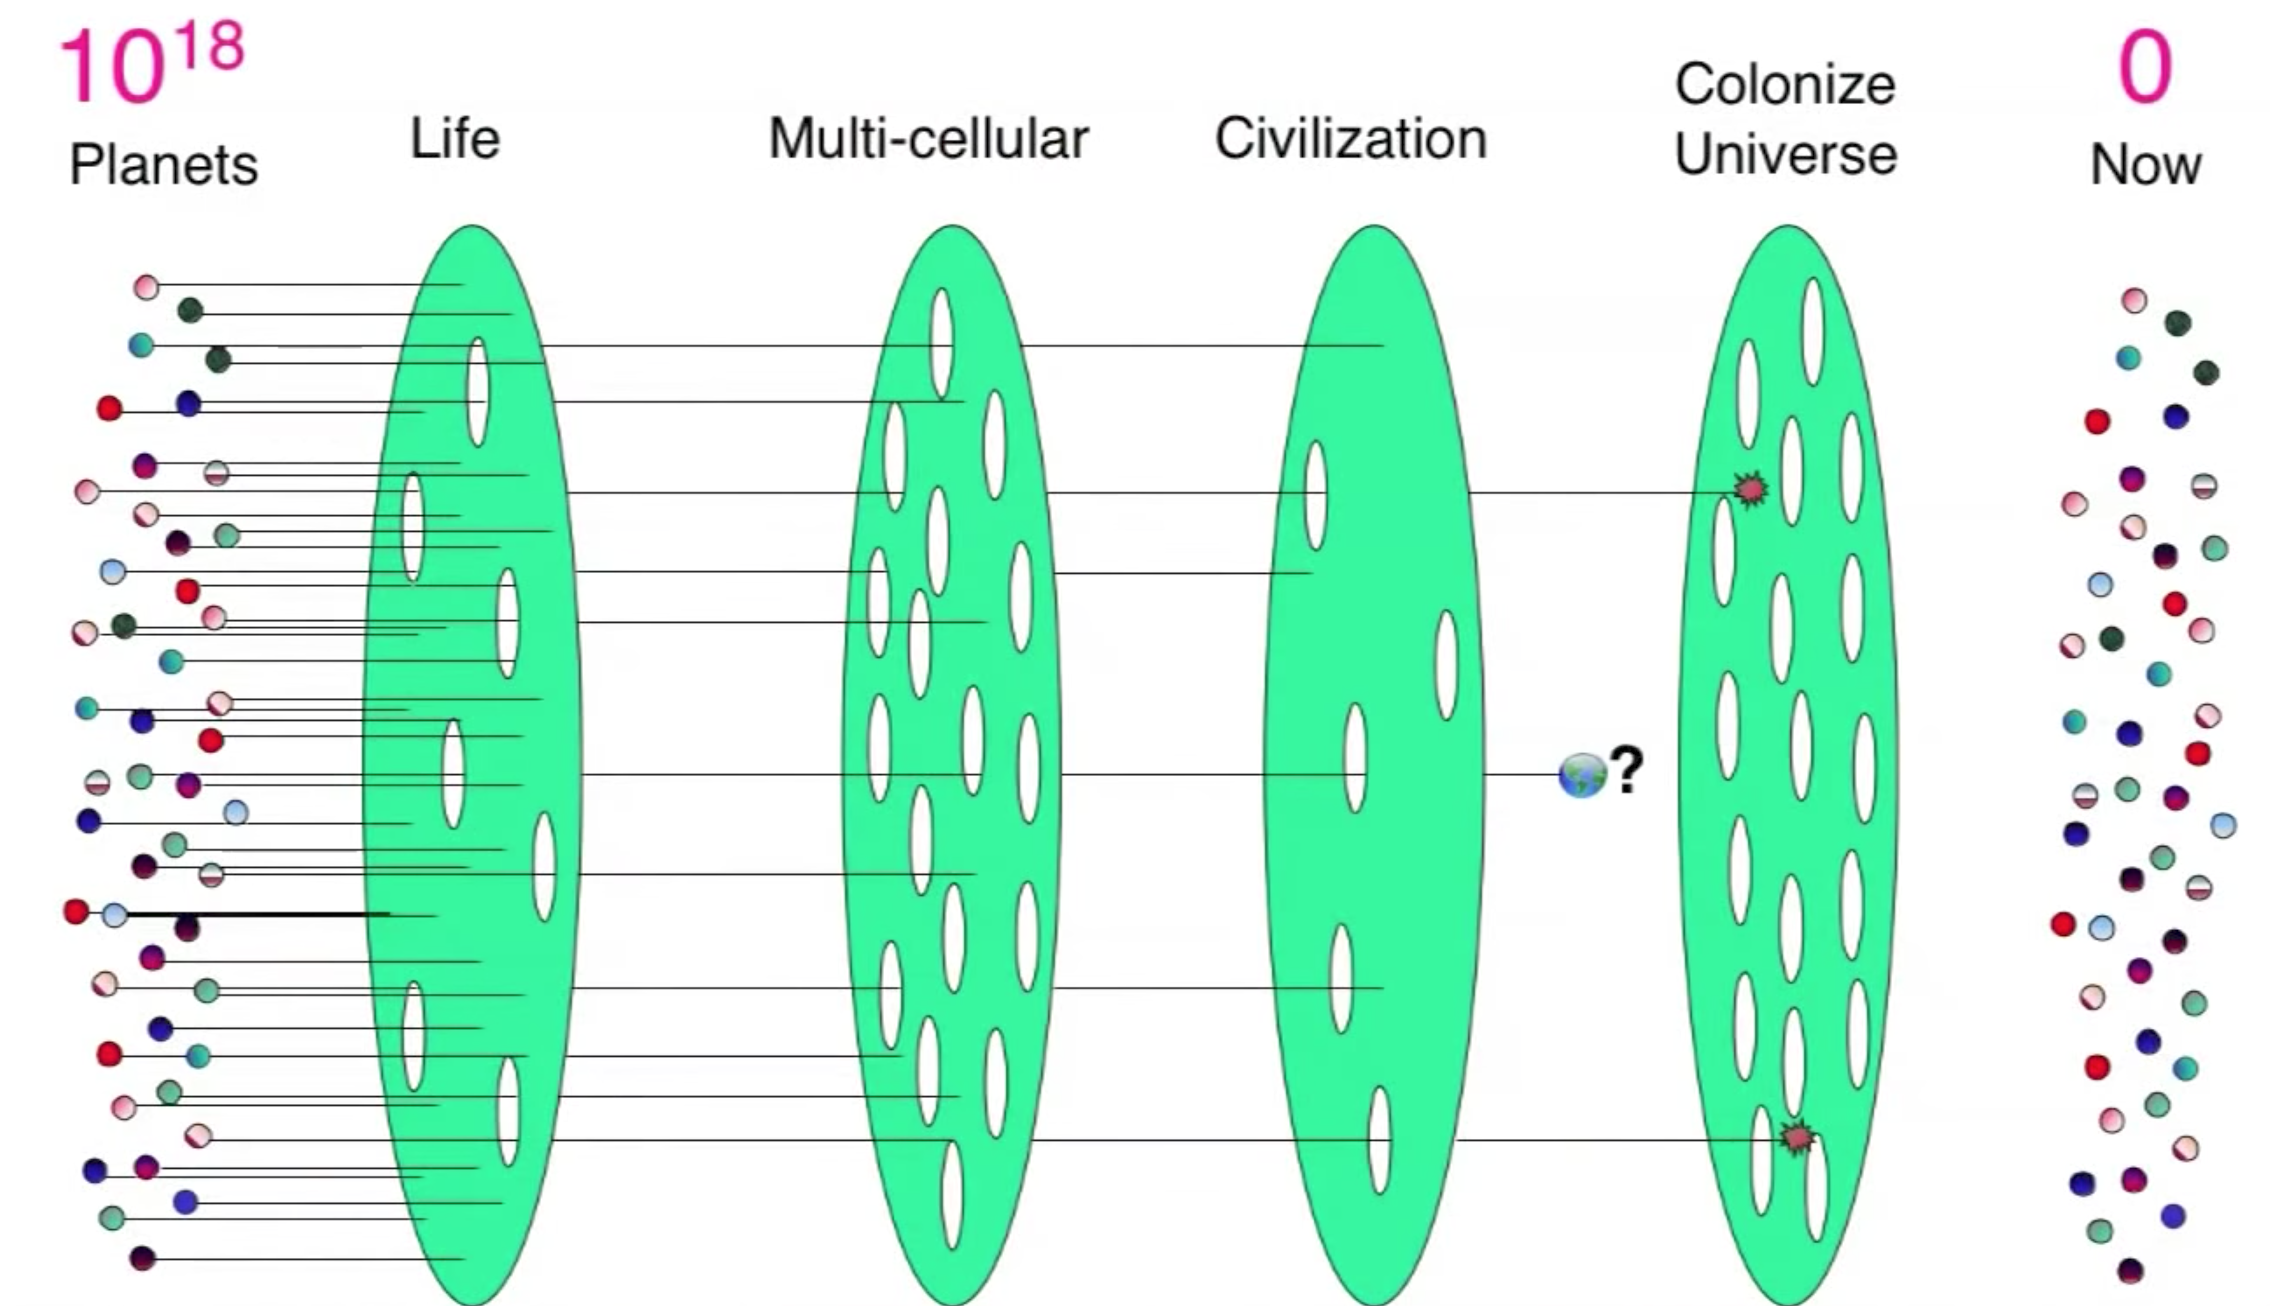
\includegraphics[width=5.35625in,height=3.20307in]{figs/great-filter}
    \caption{An illustration of the different levels of
potential filters, from Robin Hanson's
\href{https://www.youtube.com/watch?v=aspMV6ERqpo}{\emph{TEDx talk ``The
great filter''}}.}
    \label{great-filter}
\end{figure}

Filters at earlier levels would mainly make civilizations rare in
general. Late filters, on the other hand, change the distribution of
values -- value systems that more commonly lead to extinction, collapse,
or stagnation have less power than those who lead to space colonization.
The specific implications for the distribution of values depends on the
respective filter. Here are some tentative example considerations:

\begin{itemize}
\item
  If the main filter is the use of weapons of mass destruction (WMD) in
  warfare, it will favor the survival of more peaceful civilizations,
  and hence render their values more important. Civilizational traits
  that correlate with peacefulness may include
  \href{https://en.wikipedia.org/wiki/Democratic_peace_theory}{\emph{democracy}},
  \href{https://en.wikipedia.org/wiki/Nuclear_peace}{\emph{using (or not
  using) WMDs to deter conflict}},
  \href{https://en.wikipedia.org/wiki/Capitalist_peace}{\emph{capitalism}},
  having fewer internal value differences or greater tolerance thereto,
  a world government, global authoritarianism, etc. These traits may, in
  turn, correlate with particular values.
\item
  If the filter is some risk whose mitigation requires large-scale
  coordination, it will favor civilizations that are good at (causal)
  coordination problems. Such risks may include
  \href{https://en.wikipedia.org/wiki/Fermi_paradox\#Resource_depletion_and_climate_change}{\emph{global
  warming, resource depletion}}, and existential risk from research and
  technology (like
  \href{https://en.wikipedia.org/wiki/Grey_goo}{\emph{gray goo}},
  \href{https://en.wikipedia.org/wiki/Safety_of_high-energy_particle_collision_experiments}{\emph{black
  holes created in particle colliders}},
  \href{https://fas.org/sgp/othergov/doe/lanl/docs1/00329010.pdf}{\emph{nuclear
  weapons tests igniting the atmosphere}}, etc.). Similarly,
  civilizations that manage to
  \href{https://foundational-research.org/differential-intellectual-progress-as-a-positive-sum-project/}{\emph{progress
  carefully}} will likely also be favored over ones that cannot contain
  their scientific curiosity or economic growth.
\item
  If a mere lack of interest in colonizing space is a significant
  filter, then adventurous civilizations with a preference for
  colonizing space will have more influence than those who, for whatever
  reason, decide not to venture beyond their home planet.
\item
  If the filter is something that civilizations have hardly any
  influence on, such as asteroid impacts, supernovae etc., it is
  unlikely to favor any particular value system\footnote{Civilizations
    that develop protection mechanisms (like a colony on another planet)
    faster are less vulnerable to some of these risks, but these
    differences appear negligible. They could be significant in regions
    of the multiverse where, say, asteroid impacts are especially
    common, but such regions are probably too hostile for higher
    lifeforms to evolve in the first place.}.
\end{itemize}

There are further civilization-level events that cannot be used as
explanations of the Fermi paradox, but that nevertheless have similar
implications for how much power different value systems hold:

\begin{itemize}
\item
  Some
  \href{https://en.wikipedia.org/wiki/Global_catastrophic_risk}{\emph{global
  catastrophes}} may not destroy a civilization, but still change their
  values significantly. As before, this gives power to civilizations
  that can avoid value-changing catastrophes, but it also gives power to
  the value systems that result from such catastrophes.
\item
  Uncontrolled artificial intelligence (AI) does not work well as an
  explanation of the Fermi paradox, because an uncontrolled AI could
  still colonize space on its own and thereby represent a spacefaring
  civilization (if only as a rogue relic of the one that created it).
  Nevertheless, a failure to control artificial intelligence is one way
  for a civilization to lose a lot of its power. As with the other
  technological risks mentioned above, this AI filter would select for
  careful and well-coordinated civilizations. Similarly, because
  \href{https://wiki.lesswrong.com/wiki/AI_arms_race}{\emph{AI arms
  races}}
  \href{https://wiki.lesswrong.com/wiki/AI_arms_race}{w}o\href{https://wiki.lesswrong.com/wiki/AI_arms_race}{u}l\href{https://wiki.lesswrong.com/wiki/AI_arms_race}{d}
  \href{https://wiki.lesswrong.com/wiki/AI_arms_race}{m}a\href{https://wiki.lesswrong.com/wiki/AI_arms_race}{k}e
  A\href{https://wiki.lesswrong.com/wiki/AI_arms_race}{I}
  \href{https://wiki.lesswrong.com/wiki/AI_arms_race}{c}o\href{https://wiki.lesswrong.com/wiki/AI_arms_race}{n}t\href{https://wiki.lesswrong.com/wiki/AI_arms_race}{r}o\href{https://wiki.lesswrong.com/wiki/AI_arms_race}{l}
  \href{https://wiki.lesswrong.com/wiki/AI_arms_race}{e}s\href{https://wiki.lesswrong.com/wiki/AI_arms_race}{p}e\href{https://wiki.lesswrong.com/wiki/AI_arms_race}{c}i\href{https://wiki.lesswrong.com/wiki/AI_arms_race}{a}l\href{https://wiki.lesswrong.com/wiki/AI_arms_race}{l}y
  d\href{https://wiki.lesswrong.com/wiki/AI_arms_race}{i}f\href{https://wiki.lesswrong.com/wiki/AI_arms_race}{f}i\href{https://wiki.lesswrong.com/wiki/AI_arms_race}{c}u\href{https://wiki.lesswrong.com/wiki/AI_arms_race}{l}t,
  it favors the survival of
  \href{https://wiki.lesswrong.com/wiki/AI_arms_race}{p}e\href{https://wiki.lesswrong.com/wiki/AI_arms_race}{a}c\href{https://wiki.lesswrong.com/wiki/AI_arms_race}{e}f\href{https://wiki.lesswrong.com/wiki/AI_arms_race}{u}l
  c\href{https://wiki.lesswrong.com/wiki/AI_arms_race}{i}v\href{https://wiki.lesswrong.com/wiki/AI_arms_race}{i}l\href{https://wiki.lesswrong.com/wiki/AI_arms_race}{i}z\href{https://wiki.lesswrong.com/wiki/AI_arms_race}{a}t\href{https://wiki.lesswrong.com/wiki/AI_arms_race}{i}o\href{https://wiki.lesswrong.com/wiki/AI_arms_race}{n}s\href{https://wiki.lesswrong.com/wiki/AI_arms_race}{,}
  \href{https://wiki.lesswrong.com/wiki/AI_arms_race}{j}u\href{https://wiki.lesswrong.com/wiki/AI_arms_race}{s}t
  a\href{https://wiki.lesswrong.com/wiki/AI_arms_race}{s}
  \href{https://wiki.lesswrong.com/wiki/AI_arms_race}{w}i\href{https://wiki.lesswrong.com/wiki/AI_arms_race}{t}h
  \href{https://wiki.lesswrong.com/wiki/AI_arms_race}{the}
  W\href{https://wiki.lesswrong.com/wiki/AI_arms_race}{M}D
  w\href{https://wiki.lesswrong.com/wiki/AI_arms_race}{a}r\href{https://wiki.lesswrong.com/wiki/AI_arms_race}{f}a\href{https://wiki.lesswrong.com/wiki/AI_arms_race}{r}e
  f\href{https://wiki.lesswrong.com/wiki/AI_arms_race}{i}l\href{https://wiki.lesswrong.com/wiki/AI_arms_race}{t}e\href{https://wiki.lesswrong.com/wiki/AI_arms_race}{r}.
  A society with a large fraction of
  \href{https://en.wikipedia.org/wiki/Mind_uploading}{\emph{whole brain
  emulation}} citizens \parencite{Hanson2016-yn}
  \href{https://casparoesterheld.com/2016/08/30/the-age-of-em-summary-of-policy-relevant-information/\#AISafety}{\emph{may
  also}} \href{https://www.youtube.com/watch?v=Cul4-p7joDk}{\emph{be
  better at}}
  \href{https://en.wikipedia.org/wiki/Mind_uploading\#Emulation_timelines_and_AI_risk}{\emph{controlling
  AI}} (cf.
  \href{https://intelligence.org/files/SS11Workshop.pdf}{\emph{Salamon
  and Muehlhauser 2011}}; \cite{Bostrom2014-pc}),
  resulting in these societies having a higher influence than
  civilizations that directly create \emph{de novo} AI, i.e. artificial
  intelligent systems not modeled after humans or other animals.
\end{itemize}

Needless to say, these are all speculative claims which we should not
expect to have strong practical implications without further
examination. Instead, they should be seen as examples of the kind of
considerations that are necessary in order to properly estimate the
distribution of values across the multiverse.

\begin{sloppypar} % Prevents URLs from exceeding page width
\printbibliography
\end{sloppypar}
\end{document}
